\documentclass{sig-alternate}
\usepackage{epigraph}
\usepackage{amssymb}
\usepackage{mathtools}
\usepackage{tikz}
\usetikzlibrary{matrix}

\usepackage{array} 
\newcolumntype{C}{>{$}c<{$}} % math-mode version of "l" column type

\newtheorem{theorem}{Theorem}[section]
\newtheorem{lemma}[theorem]{Lemma}
\newtheorem{proposition}[theorem]{Proposition}
\newtheorem{corollary}[theorem]{Corollary}
\newtheorem{conjecture}[theorem]{Conjecture}
\newtheorem{remark}[theorem]{Remark}

\newenvironment{definition}[1][Definition]{\begin{trivlist}
\item[\hskip \labelsep {\bfseries #1}]}{\end{trivlist}}
\newenvironment{example}[1][Example]{\begin{trivlist}
\item[\hskip \labelsep {\bfseries #1}]}{\end{trivlist}}
\newenvironment{problem}[1][Problem]{\begin{trivlist}
\item[\hskip \labelsep {\bfseries #1}]}{\end{trivlist}}

\begin{document}
\onecolumn
\begin{center}\bf{\large{Misc Notes in Algebra}}\end{center}
%\title{Misc Notes}
%\maketitle
\twocolumn
\section{The Standard Representation}
Let $M_{\sigma}$ be the permutation matrix corresponding to $\sigma \in S_ns$ and let $M_{S_n}$ be the span of the $M_{\sigma}$.
\begin{lemma}
The Standard Representation of $S_n$ is irreducible. Equivalently, $dim(M_{S_n}) = n^2 -2n + 2$
\end{lemma}
\begin{proof}
Let $M_{\sigma}$ be the permutation matrix corresponding to $\sigma \in S_n$.
\begin{enumerate}
\item $dim(M_{S_n}) \leq n^2 - 2n + 2$
\begin{proof}
The permutations decompose into $\left[ \begin{array}{cc} 1 & 0 \\ 0 & M'_{\sigma} \end{array} \right]$ in a suitable basis. Alternate argument see next item.
\end{proof}
\item $dim(M_{S_n}) \geq n^2 - 2n + 2$
\begin{proof}
Define Generalized Stochastic matrices, $\mathbb{S}^{n\times n}$, as $\mathbb{R}^{n\times n}$ matrices whose row and column sums are all equal (but not necessarily 1)
\begin{enumerate}
\item $span(\{M_{\sigma}\}) \subseteq \mathbb{S}^{n\times n}$ 
\item Positive matrices in $\mathbb{S}^{n\times n} \subseteq span(\{M_{\sigma}\})$ via Birkhoff-Von Neumann. They span $\mathbb{S}^{n\times n}$. Hence, \[\mathbb{S}^{n\times n} \subseteq span(\{M_{\sigma}\})\]
\item $dim(\mathbb{S}^{n\times n}) = (n-1)^2 + 1$. Easy isomorphism $R^{(n-1)^2 + 1} \leftrightarrow \mathbb{S}^{n\times n}$
\end{enumerate}
\end{proof}
\end{enumerate}
\end{proof}

\section{Wedderburn's Theorem}
\begin{theorem}
Every finite division ring is a field
\end{theorem}
\begin{proof} Let $C_0$ be the centre of $R$. Let $q = |C_0| \geq 2$. Let $C_1, \ldots C_k$ be the conjugacy classes of $(R\backslash 0, \cdot)$.
\begin{enumerate}
\item $C_0$ is a field and $R$ is a vector space over $C_0$ with finite dimension, say $n$. It follows that $|R| = q^n$. We want to show that $n=1$.
\item For any $a \in R$ the centralizer $N(a) = \{x: xa = ax\}$ is a vector space over $C_0$. It follows that the size of the conjugacy class containing $a$ is $q^{n(a)}$ where $n(a) = |N(a)|$.
\item $N(a)\backslash 0$ is a subgroup of $(R\backslash 0, \cdot)$. It follows that the class equation can be written as
\[ q^n - 1 =  (q - 1) + \sum_{i = 1}^k\frac{q^n - 1}{q^{n_i} - 1} \mbox{ (where } n_i | n \mbox{)}\]
\item Clearly $\Phi_n(q)$ ($\Phi_n$ is $n$th cyclotomic polynomial), divides all terms above except $q-1$ so for some polynomial $p$ with integer coefficients
\begin{eqnarray*} q - 1 & = & \Phi_n(q)p(q) \\ \implies |q-1| & \geq & |\Phi_n(q)| \\ & \geq & \prod |q - \theta_i| \end{eqnarray*}
where $\theta_i$ are the primitive $n$th roots of 1. Clearly this is a contradiction if $n>1$ and $q>1$.
\end{enumerate}
\end{proof}
\section{Structure of Abelian Groups}
\begin{theorem}
Every finite abelian group $G$ of order $p^n$ can be uniquely decomposed into a product of cyclic groups of order $p^{n_1}, \ldots, p^{n_k}$ where $n_1 \geq \ldots \geq n_k$
\end{theorem}
\begin{proof} For any $s||G|$ let $G(s) = \{g \in G: g^s = 1\}$. If $G$ is cyclic then there is nothing to prove. Otherwise:
\begin{enumerate}
\item Pick an element $g_1$ in $G$ of largest order and construct $G_1 = G/\langle g_1\rangle$. Iterate till $G_k$ is cyclic.
\item $|G(s)| = p^{m_s}$ where $m_s = \sum_{i=1}^{k} \min(s, n_i)$
\item If there are distinct decompositions then there exists an $s$ such that $|G(s)|$ will be different for the two decompositions.
\end{enumerate}
\end{proof}

\section{Conjugacy Classes}
We summarize some facts for the basic groups:
\subsection{Dihedral Group}
$D_{2n} = \langle a, b\rangle$, where $a^n = 1$ and $b^{-1}ab = a^{-1}$


\section{Averaging Principle}
\begin{theorem} {\bf (Averaging Principle)}
Suppose $\rho: G \rightarrow GL(V)$ is a representation of a {\bf finite} group $G$ and $v \in V$ any vector. The vector \[\frac{1}{|G|}\sum_{g \in G}\rho(g)v\] is fixed by the action of $G$. In fact if $V_1 \subseteq V$ is the subspace of all fixed vectors for the action of $G$ then the endomorphism \[ A = \frac{1}{|G|}\sum_{g\in G}\rho(g)\] is a projection onto $V_1$.
\end{theorem}
\begin{proof} $\rho(hg) = \rho(h)\rho(g)$. The first claim follows. For the second claim,
\begin{enumerate}
\item $Im(A) = V_1$
\item If  $M^2 = M$, it is a projection operator onto $Im(M)$ \begin{proof} $v = (v - Mv) + Mv$. $(v-Mv) \in Ker(M)$.  Hence, $V = Ker(M) + Im(M)$. \\
Also, $u = Mv$ and  $Mu = 0 \implies M^2v = 0 = Mv = u$. Hence, $V = Ker(M) \oplus Im(M)$ \end{proof}
\end{enumerate}
\end{proof}

\begin{lemma}
If the minimal polynomial of $M$ has no repeated roots then $M$ is diagonalizable.
\end{lemma}
\begin{proof} $M$ is diagonalizable $\Leftrightarrow$ $M$ has an eigenbasis.
\begin{enumerate}
\item Any set of eigenvectors with distinct eigenvalues is linearly independent.
\item The direct sum of the eigenspaces is the entire space. 
\item Pick a basis for each eigenspace of $M$. 
\end{enumerate}
\end{proof}

\begin{corollary}
If $G$ is finite and  $\rho: G\rightarrow GL(V)$ is a representation then $\forall g\in G$, $\rho(g)$ is diagonalizable.
\end{corollary}

\subsection{G-action on Hom(V,W)}
\begin{definition}
Let $V,W$ be $G$-modules. We define the $G$ action on $Hom(V,W)$ as follows:
\begin{center}
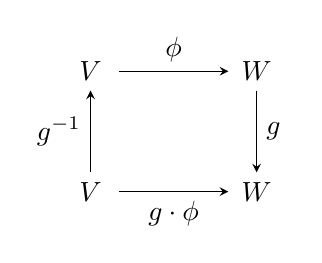
\begin{tikzpicture}
	\matrix (m) [matrix of math nodes, row sep=3em, column sep=4em, minimum width=2em] {
		V & W \\
		V & W \\};
	\path[-stealth]
		(m-2-1) edge node [left] {$g^{-1}$} (m-1-1)
		(m-1-2) edge node [right] {$g$} (m-2-2)	
		(m-1-1) edge node [above] {$\phi$} (m-1-2)
		(m-2-1) edge node [below] {$g\cdot\phi$} (m-2-2);
\end{tikzpicture}
\end{center}
\end{definition}
This turns $Hom(V,W)$ into a $G$-module.
\begin{theorem}\label{thm:avgHom}
The averaging operator:
\[A(\phi) = \frac{1}{|G|}\sum_{g\in G}g\cdot\phi \]
projects $Hom(V,W)$ onto $Hom_G(V,W)$.
\end{theorem}
\begin{proof}
The space of fixed points of the above $G$-action is $Hom_G(V,W)$. 
\begin{eqnarray*}
g\phi g^{-1} = \phi &  \Longleftrightarrow & g\phi = \phi g \\
 & \Longleftrightarrow & \forall(v \in V)\mbox{, } g\cdot \phi(v) = \phi(g\cdot v) \\
 & \Longleftrightarrow & \phi \in Hom_G(V,W)
 \end{eqnarray*}

It follows from the averaging principle, that the operator $A$ is a projection onto $Hom_G(V,W)$
\end{proof}

Note the different objects types:
\begin{enumerate}
\itemsep0em
\item $G$-modules $V$, $W$
\item Vector space $Hom(V,W)$
\item $G$-module $Hom(V,W)$ using the $G$-action defined
\item Vector subspace $Hom_G(V,W)$ of $Hom(V,W)$. $G$ acts trivially on this.
\end{enumerate}

\subsection{G-invariant inner product}
\begin{lemma}
If $G$ is a group and $\rho: G\rightarrow GL(V)$ is a finite dimensional representation. Then $\exists$ an inner product on $V$ that is preserved by the action of $G$.
\end{lemma}
\begin{proof}
Choose any basis $\mathbb{B} = (v_1, \ldots, v_n)$ of $V$ and let $\langle,\rangle_{\mathbb{B}}$ be the corresponding inner product. We define
\[ [v_1, v_2]_{\mathbb{B}} = \frac{1}{|G|}\sum_{g \in G} \langle gv_1, gv_2\rangle_{\mathbb{B}}\]
Clearly,
\begin{eqnarray*}
[hv_1, hv_2]_{\mathbb{B}} & = & \frac{1}{|G|}\sum_{g \in G} \langle ghv_1, ghv_2\rangle_{\mathbb{B}} \\
& = &\frac{1}{|G|}\sum_{g \in G} \langle gv_1, gv_2\rangle_{\mathbb{B}} \\
& = & [v_1, v_2]_{\mathbb{B}}
\end{eqnarray*}
\end{proof}

\subsection{R-module complements}
Let $R$ be a ring and $N\leq M$ be left $R$-modules. The following lemma shows that a complement of $N$ in $M$ is simply a system of coset representatives of $M/N$ that is itself an $R$-module:
\begin{lemma}
$R$-module complements of $N$, if they exist, are unique up to isomorphism. In fact if,
\[ M = N \oplus N_1 = N \oplus N_2 \]
then,
\[N_1 \cong N_2 \cong M/N \mbox{ canonically} \]
\end{lemma}
\begin{proof}
Consider the restriction $\phi |_{N_1}$ of the canonical map $\phi :M\rightarrow M/N$ to $N_1$. Clearly,
\[Ker(\phi |_{N_1}) = N\cap N_1 = \{0\}  \mbox { hence } \phi |_{N_1} \mbox{ is injective } \]
For any $\alpha \in M/N$, pick an $a\in\alpha$.
\begin{eqnarray*} 
M = N \oplus N_1 & \Longrightarrow & a = n + n_1, n\in N, n_1\in N_1 \\
 & \Longrightarrow  & \alpha = n_1 + N \\
& \Longrightarrow & \phi |_{N_1}(n_1) = \alpha \\
& \Longrightarrow & \phi |_{N_1} \mbox{ is surjective}
\end{eqnarray*} 
\end{proof}

\begin{lemma}
Suppose $N$ has an $R$-module complement $N_{\alpha}$. All complements of $N$ are in bijection with homomorphisms $\phi\in Hom_R(N_{\alpha}, N)$ given by $N_{\phi} = \{ \phi(x) +  x : x \in N_{\alpha} \}$.
\end{lemma}
\begin{proof}
Suppose $N_{\beta}$ a system of coset respresentatives and $\theta:N_{\alpha}\rightarrow N_{\beta}$ as below:
\begin{center}
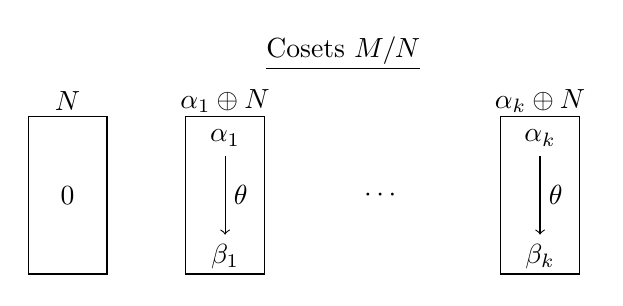
\begin{tikzpicture}
  \draw (4,2.8) node {\underline{Cosets $M/N$}};
  \draw (0.5,2.2) node {$N$};
  \draw (0,0) rectangle (1,2);
  \draw (0.5,1) node {$0$};

  \draw (2.5,2.2) node{$\alpha_1 \oplus N$};
  \draw (2,0) rectangle (3,2);
  \draw[->] (2.5,1.5) node[above] {$\alpha_1$} --
   (2.5,0.5) node[below] {$\beta_1$};
  \draw (2.7, 1) node{$\theta$};
  
  \draw (4.5, 1) node {$\cdots$};
  
  \draw (6.5,2.2) node{$\alpha_k \oplus N$};
  \draw (6,0) rectangle (7,2);
  \draw[->] (6.5,1.5) node[above] {$\alpha_k$} --
  (6.5,0.5) node[below] {$\beta_k$}; 
  \draw (6.7, 1) node{$\theta$};
\end{tikzpicture}
\end{center}
Consider the map $\phi = \theta - I$. Clearly $Im(\phi) \subseteq N$.
\begin{eqnarray*}
M = N \oplus N_{\beta} & \Longleftrightarrow & \theta \in Iso_R(N_{\alpha}, N_{\beta})  \mbox{ (previous lemma)}\\
 & \Longleftrightarrow & \phi \in Hom_R(N_{\alpha}, N)
 \end{eqnarray*} 
%Clearly, $N_{\phi}$ is an $R$-submodule of $M$, and for any $m\in M$
%\begin{eqnarray*}
%m & = & n + \bar{n} \mbox{, } n\in N, \bar{n} \in \bar{N} \\
%& = & (n - \phi(\bar{n})) + (\phi(\bar{n}) + \bar{n})
%\end{eqnarray*}
%Also,
%\begin{eqnarray*}
%(\phi(x) + x \in N) & \Longleftrightarrow &(x = 0) \\
%\Rightarrow N \cap N_{\phi} & = & \varnothing \\
%\Rightarrow M  & = & N \oplus N_{\phi}
%\end{eqnarray*}
%Conversely, if there exists a complement $N' \neq \bar{N}$, the previous lemma gives us an isomorphism $\theta:\bar{N}\rightarrow N'$.
\end{proof}

\begin{corollary}
In the above lemma
\[ (Hom_R(N_{\alpha}, N) = \{0\}) \Longleftrightarrow (N_{\alpha} \mbox{ is uniquely defined}) \]
\end{corollary}

\subsection{Complements in $\mathbb{C}G$}
\begin{theorem} [Maschke]
Let $G$ be a finite group and $V$ a $\mathbb{C}G$-module. $V$ is a direct sum $V_1\oplus\cdots\oplus V_k$ where the $V_i$ are simple.
\end{theorem}
\begin{proof}
Enough to show that for any proper submodule $U \subseteq V$ there is a decomposition $V = U \oplus W$.
\begin{enumerate}
\item First proof: 
   \begin{enumerate}
   \item Extend any basis of $U$ to a basis $\mathbb{B}$ of $V$.
   \item Pick $W = U^{\perp}$ wrt the inner product $[,]_{\mathbb{B}}$. It only remains to check that $W$ is closed under $G$-action:
       \begin{eqnarray*}
       [w, u]_{\mathbb{B}} & = & 0 \mbox{, }\forall u \in U\\
       \implies [hw, u]_{\mathbb{B}} & = &  \frac{1}{|G|}\sum_{g \in G} \langle ghw, gu\rangle_{\mathbb{B}} \\
       & = & [w, h^{-1}u]_{\mathbb{B}} \\
       & = & 0
       \end{eqnarray*}
    \end{enumerate}
 \item Second proof:
    \begin{enumerate}
    \item Extend any basis of $U$ to a basis of $V$ and define the projection $\phi$ onto $U$ in this basis.
    \item The averaged operator (using the G-action in previous section), $\phi_A$, is a $\mathbb{C}G$-module projection onto $U$.
    \item $W = Ker(\phi_A)$
    \end{enumerate}
\end{enumerate}
\end{proof}

\begin{lemma}
For any $\mathbb{C}G$-module $V$, the isotypic component of the one dimensional trivial representation in $V$ is unique.
\end{lemma}
\begin{proof}
Let,
\[ V = c_1U_1 \oplus \cdots \oplus c_kU_k \]
where $c_iU_1$ is the isotypic component of the 1D trivial representation, and let
\[ F = \{v : v\in V \mbox{ and } g\cdot v = v\}\]
Clearly $v\in c_1U_1 \Rightarrow v\in F$
Now suppose $v\in F$ and
\begin{eqnarray*}
v & = & \sum_{1\leq i\leq k} v_i \mbox{  where } 0\neq v_i \in c_iU_i \\
\Rightarrow g\cdot v & = & \sum_{1\leq i\leq k} g\cdot v_i  \mbox{, }\forall g\in G
%\Rightarrow g\cdot (v - v_1) & = & \sum_{1< i\leq k} g\cdot v_i  \mbox{, }\forall g\in G
\end{eqnarray*}
Since $G$ does not act trivially on $c_iU_i$ ($i\ne 1$)there must exist $v_i \neq 0$. For this $v_i$ there must be a $g\in G$ such that $g\cdot v_i \neq v_i$. 
\end{proof}
\begin{corollary}
The projection onto $V_1$ in the averaging principle is unique.
\end{corollary}

\begin{theorem}
For any $\mathbb{C}G$-module $V$ and irreducible $\mathbb{C}G$-module $U$, the isotypic component of $U$ in $V$ is unique.
\end{theorem}
\begin{proof}
Suppose $U_1, U_2$ are distinct isotypic components of $U$ in $V$.
\begin{enumerate}
\item From Maschke's theorem, $V = U_1 \oplus V_1$. Consider any projection of $U_2$ into $V_1$.
\item Schur's theorem ensures that the image of this projection is $\{0\}$, hence $U_2 \subseteq U_1$.
\item Other direction is similar.
\end{enumerate}
\end{proof}

\subsection{Inner product of characters}
We start with a simple restatement of the averaging principle:
\begin{lemma}
Let $G$ be a group and $\mathbb{C}$ be its trivial 1D representation. For any representation $U$ of $G$,
\[ dim(Hom_G(\mathbb{C}, U)) =  \langle\chi_{\mathbb{C}}, \chi_U\rangle \]
\end{lemma}
\begin{proof}
Clearly, $Hom(\mathbb{C}, U) \cong U$ as vector spaces. Let $\phi_u \in Hom(\mathbb{C}, U)$ take 1 to $u$. The following diagram:
\begin{center}
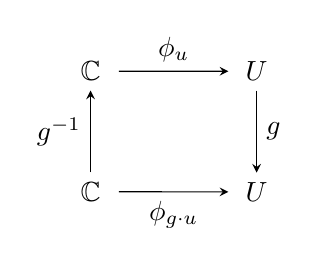
\begin{tikzpicture}
	\matrix (m) [matrix of math nodes, row sep=3em, column sep=4em, minimum width=2em] {
		\mathbb{C} & U \\
		\mathbb{C} & U \\};
	\path[-stealth]
		(m-2-1) edge node [left] {$g^{-1}$} (m-1-1)
		(m-1-2) edge node [right] {$g$} (m-2-2)	
		(m-1-1) edge node [above] {$\phi_u$} (m-1-2)
		(m-2-1) edge node [below] {$\phi_{g\cdot u}$} (m-2-2);
\end{tikzpicture}
\end{center}
\noindent shows that the $G$-representations on $Hom(\mathbb{C}, U)$, and $U$ are isomorphic (say $\rho$)\\

\noindent Consider the averaging operator $A$ from theorem \ref{thm:avgHom} acting on $Hom(\mathbb{C}, U)$:
\begin{eqnarray*}
dim(Hom_G(\mathbb{C}, U)) & = & Tr(A) \\
& = & \frac{1}{|G|}\sum_{g\in G}Tr(\rho(g)) \\
& = &  \frac{1}{|G|}\sum_{g\in G}\chi_U(g) \\
& = & \langle\chi_{\mathbb{C}}, \chi_U\rangle
\end{eqnarray*}
\end{proof}

\noindent The following theorem is just a generalization of the averaging principle:
\begin{theorem}
Let $U,V$ be representations of a group $G$ and $\chi_U, \chi_V$ their respective characters.
\[ \langle\chi_U, \chi_V\rangle = dim(Hom_G(U,V)) \]
\end{theorem}
\begin{proof}
Let $\rho_U, \rho_V$ be the representations of $G$ in $U,V$ respectively.
Clearly, for $M\in Hom(U,V)$ and $g\in G$,
\[ g\cdot M = \rho_V(g)M\rho_U(g)^{-1} =  \rho_V(g)M\rho_U(g^{-1}) \]
Let $\rho$ be the representation of $G$ in $Hom(U,V)$, $\chi$ its character and $E_{i,j}$ the standard basis of $Hom(U,V)$.
\begin{eqnarray*}
Tr(\rho(g)) & = & \sum_{i,j}(\rho_U(g^{-1}))_{i,i}(\rho_V(g))_{j,j} \\
& = & Tr(\rho_U(g^{-1}))\cdot Tr(\rho_V(g)) \\
\Rightarrow \chi_(g^{-1}) & = & \chi_U(g)\cdot \chi_V(g)
\end{eqnarray*}
Using the previous lemma on the representation $\rho$,
\begin{eqnarray*}
dim(Hom_G(\mathbb{C}, Hom(U,V)) & = & \frac{1}{|G|}\sum_{g\in G}\chi(g) \\
\Rightarrow dim(Hom(U,V)) & = & \frac{1}{|G|}\sum_{g\in G}\chi_U(g^{-1})\cdot \chi_V(g) \\
& = & \langle\chi_U, \chi_V\rangle
\end{eqnarray*}
\end{proof}

\section{R-Module Homomorphisms}
Let $R \leq S$ be rings, $M,N$ be $R$-modules.
\begin{enumerate}
\item $Hom_R(M,N)$ is an $R$-module iff $R$ is commutative
\item $Hom_R(R, M) \cong M$ as abelian groups
\item Every $\phi \in Hom_R(R, S)$ is the right multiplication by $\phi(1)$.
\item $Hom_R(R,R) \cong R^{opp}$ as rings
\end{enumerate}

\subsection{Homomorphisms in $\mathbb{C}G$}
Let $H \leq G$ be groups and $U$ be a left $\mathbb{C}H$-submodule of $\mathbb{C}H$.
\begin{enumerate}
\item Any $\phi \in Hom_H(U, \mathbb{C}H)$ is given by right multiplication by  some $\alpha \in \mathbb{C}H$
\begin{proof}
By Maschke's Theorem, $\mathbb{C}H = U \oplus  V$ for some $\mathbb{C}H$-submodule $V$. Let $\psi$ be a projection operator, $\psi:\mathbb{C}H \rightarrow U$. 
\end{proof}

\end{enumerate}

\section{Induced Representations}
Let $H\leq G$ be groups and let $U$ be a $\mathbb{C}H$-module with $H$ action given by $\rho$ and character $\chi$. We give three equivalent definitions of the induced $\mathbb{C}G$-module $U\uparrow G$, equivalently the induced representation $\rho\uparrow G$ and induced character $\chi\uparrow G$
\begin{definition} [Definition I1]
Choose a system of left coset representatives $g_1=1, \ldots, g_k$ of $H$ in $G$. Extend $\rho$ by defining $\rho(g) = 0$ whenever $g\in G\setminus H$. Similarly $\chi$.
\[ (\rho\uparrow G)(x) =
\begin{bmatrix}
\rho(g_1^{-1}xg_1) & \rho(g_1^{-1}xg_2) & \cdots & \rho(g_1^{-1}xg_k) \\
\rho(g_2^{-1}xg_1) & \rho(g_2^{-1}xg_2) & \cdots & \rho(g_2^{-1}xg_k) \\
\vdots & \vdots & \rho(g_i^{-1}xg_j) & \vdots \\
\rho(g_k^{-1}xg_1) & \rho(g_k^{-1}xg_2) & \cdots & \rho(g_k^{-1}xg_k) \\
\end{bmatrix}
\]

\begin{eqnarray*}
(\chi\uparrow G)(x) & = & \sum_i \chi(g_i^{-1}xg_i)  \\
& = & \frac{1}{|H|}\sum_{g\in G}  \chi(g^{-1}xg)
\end{eqnarray*}
Note that this definition allows us to extend the definition of $\chi\uparrow G$ to any class function $\chi$.
\end{definition}

\begin{definition}[Definition I2]
Choose a system of left coset representatives $g_1=1, \ldots, g_k$ of $H$ in $G$. Let $e_1, \ldots, e_l$ be a basis of $U$. We construct the vector space with basis symbols $g_i\otimes e_j$ with the following properties:
\begin{enumerate}
\item $h\otimes e_j = 1\otimes he_j$, whenever $h\in H$
\item $g_i\otimes (\sum_j c_je_j) = \sum_j c_j g_i \otimes e_j$ 
\item $g\cdot (g_i\otimes e_j) = g_a\otimes he_j$, where $gg_i = g_ah$
\end{enumerate}
\end{definition}
{\bf Note}: Add "extension of scalars definition"

\begin{theorem}[Frobenius' Reciprocity Theorem]
Let $\chi, \psi$ be any class functions on $H, G$ respectively.
\[ \langle\chi\uparrow G, \psi\rangle_G = \langle\chi, \psi\downarrow H\rangle_H \] 
\end{theorem}

\begin{proof}
Bilinearity of inner product ensures that it is enough to verify for arbitrarily chosen bases of the space of class functions over $H, G$. We choose the bases of indicators of the conjugacy classes in $H, G$.

Fix $h_0\in H, g_0\in G$ and let
\[\chi = \mbox{indicator of } h_0^H,\hspace*{0.4cm}  \psi = \mbox{indicator of } g_0^G \]
Suppose $x\in h_0^G$,
\begin{eqnarray*}
(\chi\uparrow G)(x) & = & \frac{1}{|H|}\sum_{g\in G}\chi(g^{-1}xg) \\
& = & \frac{|C_G(x)|\cdot |h_0^H|}{|H|} \\
& = & \frac{|C_G(x)|}{|C_H(h_0)|} \\
& = & \frac{|C_G(h_0)|}{|C_H(h_0)|}
%\Rightarrow  \langle\chi\uparrow G, \psi\rangle_G
\end{eqnarray*}
Hence we have,
\[ (\chi\uparrow G)(x) = \begin{cases} \frac{|C_G(h_0)|}{|C_H(h_0)|} & \text{if } x\in h_0^G \\ 0 & \text{otherwise}\end{cases} \]
Also note,
\[ (\psi\downarrow H)(x) = \begin{cases} 1 & \text{if } x\in h_0^G \\ 0 & \text{otherwise}\end{cases} \]
Finally,
\begin{eqnarray*}
\langle\chi\uparrow G, \psi\rangle_G & = & \frac{1}{|G|}\sum_{g\in G}(\chi\uparrow G)(g)\cdot \psi(g) \\
& = & \frac{1}{|G|}\cdot  \frac{|C_G(h_0)|}{|C_H(h_0)|} |h_0^G| \\
& = & \frac{1}{|C_H(h_0)|} \\
\langle\chi, \psi\downarrow H\rangle_H & = &  \frac{1}{|H|}\sum_{h\in H}\chi(h)\cdot (\psi\downarrow H)(h) \\
& = & \frac{|h_0^H|}{|H|} \\& = &  \frac{1}{|C_H(h_0)|}
\end{eqnarray*}
\end{proof}
\end{document}